\section{Fundamental HPC and performance assessment terms}
\label{section:terminology:hpc-terms}


We try to keep the HPC jargon in this write-up to a minimum.
You might argue that this is a bad idea as we want to run scientifically sound
assessments.
However, we have to acknowledge that most scientific code today is written by
people without a computer science background, and that most scientists do not
have an extensive HPC training.
It is therefore not only a matter of accessibility of the performance analysis
and assessment itself to try to avoid too much jargon---if we use too much of
it, we run risk that our outputs, i.e.~the assessments themselves, cannot be
read and interpreted appropriatedly by our target audience.
After all, most of the assessments are not done for ourselves, but for other
scientists.


At the same time, performance analysis tools are written by computer scientists,
software stacks are written by computer scientists, and computer hardware is
built by computer scientists.
It is hence clear that there's a lot of jargon buried in any conversation around
performance. 
We have to find a healthy middle ground to make precise, in-depth assessments
and analyses, without immersing ourselves in technical fuzz.



\paragraph{Performance assessment vs.~analysis}


\paragraph{Some of the most important performance analysis terms}

\index{Profiling}
\index{Tracing}
When we speak of \emph{profiling}, we mean recording and presenting (accumulated) metrics. 
The classic example is measuring how much time we spend in a function or waiting for a message to arrive. 
\emph{Tracing} is the counterpart to profiling. 
Here, we record performance data of individual events.
We are interested in the sequence of operations occurring within the system.
Profiling focuses on the effect of program execution while tracing focuses on
the source of behaviour (Figure~\ref{figure:hpc-terms:profiling-tracing}).
Many developers confuse these definitions, which we took from the VI-HPS
community \cite{}.


\index{Tracing!Filtering}
Tracing can certainly be used to generate profiles, provided the recorded performance data encompasses all quantities required for a particular metric. 
Conversely, the reverse problem is ill-defined—it is generally impossible to reconstruct a trace from a profile without specialized knowledge of the code's internal workings.
One might immediately ask why we don't trace all the time. 
The answer is equally obvious: 
It is too expensive. 
Tracing generates enormous amounts of data. 
Therefore, all real-world tracing relies heavily on filtering, where you determine beforehand which types of
events to trace, which quantities to measure, and which program parts to monitor. 
Consequently, we revise our introductory statement:
most traces are \emph{not} well-suited for deriving program metrics, as they are, by definition, incomplete.


\index{Profiling!Sampling}
To create a profile, we distinguish between two techniques: 
We can \emph{sample} program execution. 
Essentially, we run the code, pause it at regular intervals, and each time examine our metric of interest at that point. 
Over time, we gather a good impression of which functions are called most
frequently, how many MFlops/s we achieve, and so forth. 
As with all statistical methods, the data quality improves the longer an application runs. 
However, the risk of missing important but brief effects remains.


\begin{figure}[htb]
 \begin{center}
  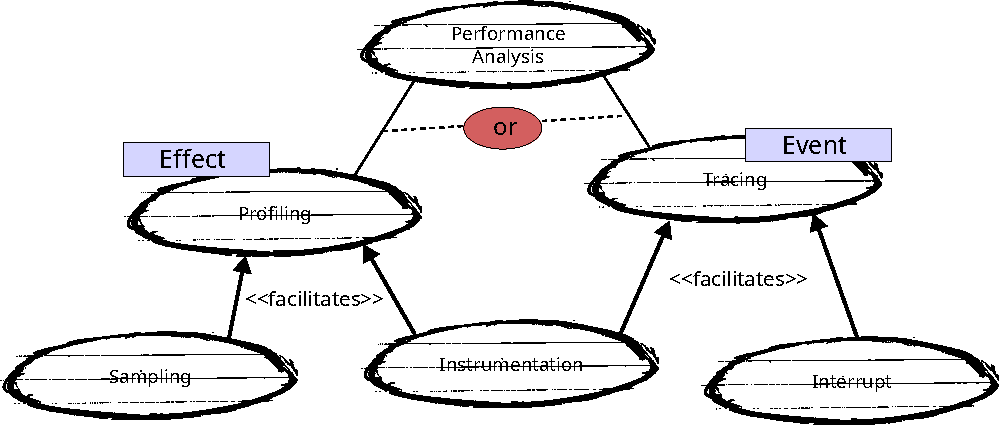
\includegraphics[width=0.85\textwidth]{terminology/profiling-tracing.pdf}
 \end{center}
 \caption{
  Overview of some fundamental performance analysis concepts.
  \label{figure:hpc-terms:profiling-tracing}
 }
\end{figure}

\index{Profiling!Instrumentation}
Alternatively, we can \emph{instrument} an application. 
Instrumentation involves inserting measurement code into our actual code which then measures quantities of interest whenever these insertion points are reached. 
We can insert either at compile time, or in a postprocessing step after the compile, or alter the code as we go.
Instrumentation yields very accurate data
(provided we instrument all relevant code sections), but it can become prohibitively expensive.


\index{Profiling!Exclusive}
\index{Profiling!Inclusive}
Most functions in our applications call other functions. 
Therefore, we must always clearly state whether any metric we present (e.g.,
runtime) is \emph{inclusive}, comprising all contributions from called routines, or \emph{exclusive}, representing only the function itself.



\index{Hardware counters}
When tracking metrics, measuring time and call frequency is straightforward:
we either measure system time or simply count occurrences. 
Other metrics are more complicated to obtain. 
Fortunately, modern systems offer performance counters.
They are special registers within the chip that automatically count certain
events.
For example, they can be configured to count every floating-point operation or every main memory access, allowing us to sample them or read their values upon completion. 
Performance counter registers are expensive to manufacture, so they are limited in number, and not every vendor tracks all possible events. 
Consequently, some analyses might not be possible on every system, and complex analyses might require multiple code executions, as only a few event types can be measured per run.



\paragraph{Hardware jargon}

We revise the bare minimum of hardware jargon here to get started, and then
refer to further resources to revise details.


\index{Node}
Supercomputers consist of many different individual computers linked through a
high-performance interconnect (network).
These computers are called \emph{nodes}.


\index{Core}
\index{Hardware thread}
Each node is a full-grown computer and hence hosts many individual \emph{cores}.
All the cores on a node share their memory (but cores from different nodes do
typically not share memory).
Technically, many vendors call their cores \emph{hardware threads}, as a core
is a technical building block and might host multiple threads. 
We use hardware thread and core as synonym.


On larger systems, you do not use the compute nodes directly.
Instead, you log into a \emph{login node}, you compile your code there, and
then you hand your code over to a \emph{scheduler}.
The most popular scheduler today is Slurm.
Slurm takes your request, i.e.~how many nodes you want to have and for how long,
as well as all the other requests from all other users and puzzles out a fair
and efficient way to assign the resources.
For performance analysis, it makes sense to investigate if your system of choice
offers a test or benchmarking queue with a high priority.
These queues usually offer only a few nodes and restrict the maximum application
runtime.
In return, jobs handed over to these queues are scheduled with high priority.


Compilation should be on the login node, as the actual compute nodes might not
provide all the required software, and many production nodes are also shielded
from the Internet, i.e.~even updating you repository is pain.
Benchmarking should not be done on the login nodes, as you share them with all
other users. 
In contrast, you can tell the scheduler that you want to have nodes
\emph{exclusive}, so no other user interfers with your measurements.
This is particularly important for all data stemming from performance counters,
as these counters are a hardware feature that we read out, i.e.~our profiler or
tracer cannot distinguish if a hardware counter's data stems from your code or
another code if multiple users coexist on one machine.



\paragraph{Core performance quantities}
\label{section:terminology:hpc-terms:core-terms}

\index{Speedup}
The runtime of a code is written here as $t(p)$ where the $p$ is either the
number of nodes or number of cores.
It depends on the context.
The \emph{speedup} of a program is defined as 

\begin{equation}
  \label{equation:hpc-terms:speedup}
  S(p) = \frac{t(1)}{t(p)},
\end{equation}

\noindent
which is typically smaller or equal to one and tells us how much faster we made
an application by using $p$ compute units (cores or nodes) rather than only one.

\index{Parallel efficiency}
The \emph{parallel efficiency} is given by 

\begin{equation}
  \label{equation:hpc-terms:efficiency}
  E(p) = \frac{S(p)}{p}.
\end{equation}

\noindent
It quantifies to which degree adding further compute resources was worth it.


\paragraph{Further material}
